% !TeX encoding = UTF-8
\documentclass[12pt,A4paper,titlepage]{article}
\usepackage[spanish]{babel}
\usepackage[utf8]{inputenc} %Este paquete permite poner acentos directamente y ees
\usepackage[T1]{fontenc}
\usepackage{amsmath}
\usepackage{graphicx}%[pdftex]
\usepackage{graphicx, wrapfig}
\usepackage{fancyhdr}
\usepackage{anysize}
\usepackage{verbatim}
\usepackage[dvips,final]{epsfig}
\usepackage{epstopdf}
\usepackage{colortbl}
\usepackage{listings}
\usepackage{float}
\usepackage{color}
\usepackage{url}
\marginsize{2.5cm}{2.5cm}{2.5cm}{2.5cm}
\usepackage{fancyhdr}
\pagestyle{fancy}
\fancyhf{}
\fancyhead[LO]{Arquitectura de Computadoras}
\fancyfoot[LE,RO]{\thepage}
\fancyfoot[LO]{Aagaard Martín - Navarro Matias}
\renewcommand{\footrulewidth}{0.4pt}

\setcounter{tocdepth}{5} % if you want all the levels in your table of contents

%\graphicspath{{figuras/}}

%defiino un estilo de ingreso de codigo
\definecolor{codegreen}{rgb}{0,0.6,0}
\definecolor{codegray}{rgb}{0.5,0.5,0.5}
\definecolor{codepurple}{rgb}{0.58,0,0.82}
\definecolor{backcolour}{rgb}{0.95,0.95,0.92}
 
\lstdefinestyle{mystyle}{
    backgroundcolor=\color{backcolour},   
    commentstyle=\color{codegreen},
    keywordstyle=\color{magenta},
    numberstyle=\tiny\color{codegray},
    stringstyle=\color{codepurple},
    basicstyle=\footnotesize,
    breakatwhitespace=false,         
    breaklines=true,                 
    captionpos=b,                    
    keepspaces=true,                 
    numbers=left,                    
    numbersep=5pt,                  
    showspaces=false,                
    showstringspaces=false,
    showtabs=false,                  
    tabsize=2
}
\lstset{style=mystyle}
\setlength{\parindent}{1cm}
\setlength{\parskip}{\baselineskip} 

\begin{document}
\renewcommand{\tablename}{Tabla}
\large

\title{Arquitectura de Computadoras \\
\large Trabajo Páctico Nº4 - MIPS}
\author{Aagaard Martin - Navarro Matias
\bigskip
\bigskip}

\date{Universidad Nacional de Córdoba \\ 27 de noviembre de 2019}

\begin{titlepage}
\center


\begin{figure}[h]
    \centering
    
\includegraphics[scale=0.8]{figure/logos-fcefyn-y-unc.png}
    \label{fig:unc-logo}
\end{figure}

{\let\newpage\relax\maketitle}
\center
\end{titlepage}

\maketitle % Compila la carátula
\tableofcontents % Arma el índice
\newpage

\section{Introducción}
Para el Trabajo Final de la materia, se realizó la implementación en Verilog del pipeline de cinco etapas del procesador \textbf{MIPS}. El mismo se trata de un procesador de 32 bits, con 32 registros, una memoria de instrucciones de 2048 posiciones y una memoria de datos de 1024 posiciones.
El mismo fue desarrollado mediante lenguaje de especificación de hardware Verilog y haciendo uso del entorno de desarrollo Vivado.



\section{Objetivos}
\noindent Las etapas se definieron según muestra la figura \ref{fig:div-mips}:

\begin{figure} [H]
    \centering
    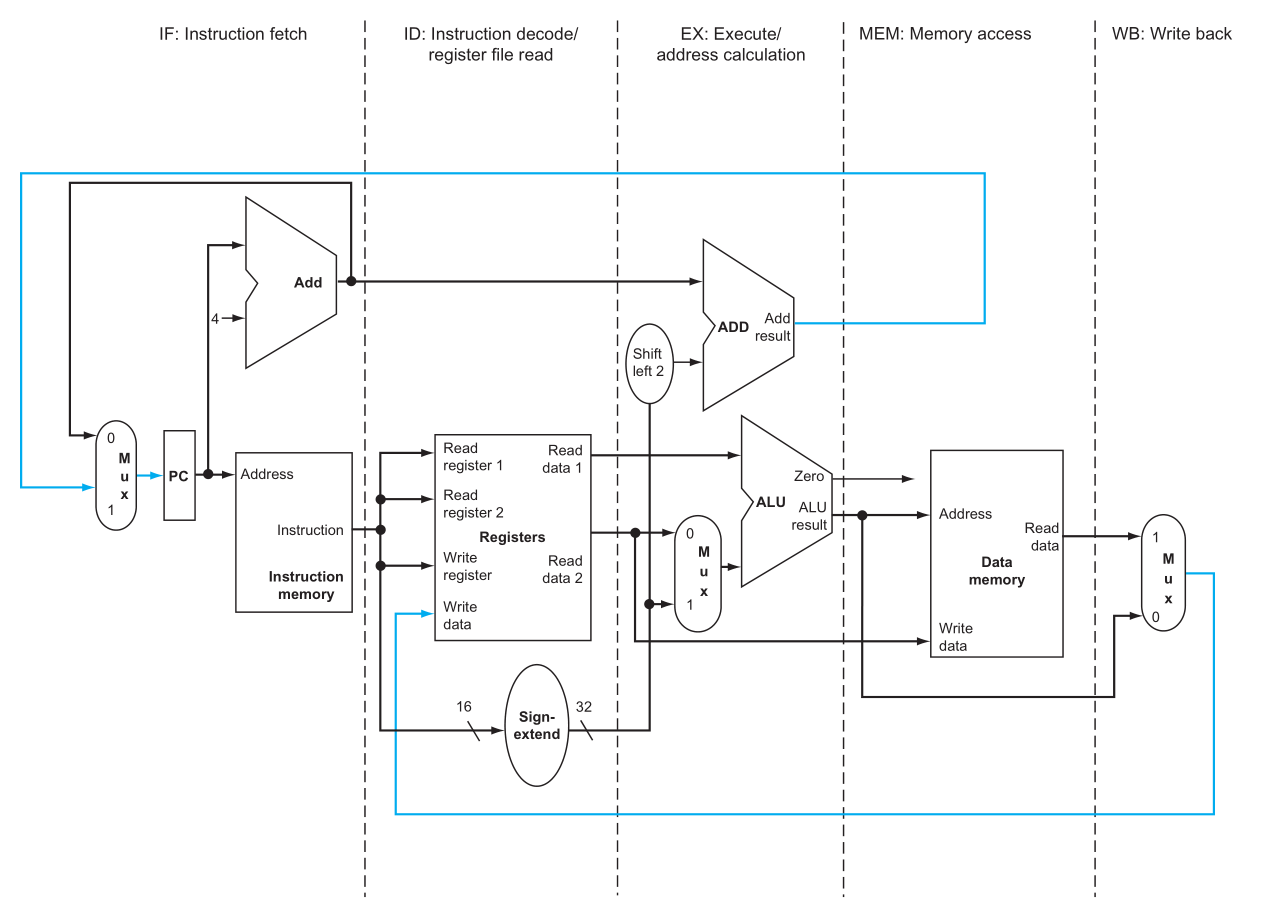
\includegraphics[width=\textwidth]{figure/figure433-mips-segmentado-basico.png}
    \caption{División del MIPS.}
    \label{fig:div-mips}
\end{figure}

\begin{itemize}
    \item \textbf{IF (Instruction Fetch)}: búsqueda de la instrucción en la memoria de programa.
    \item \textbf{ID (Instruction Decode)}: decodificación de la instrucción y lectura/escritura de
    registros.
    \item \textbf{EX (Execute)}: ejecución de la instrucción propiamente dicha.
    \item \textbf{MEM (Memory Access)}: lectura o escritura desde/hacia la memoria de datos.
    \item \textbf{WB (Write back)}: escritura de resultados en los registros.
\end{itemize}



\noindent Las instrucciones a implementar del set de instrucciones del MIPS son las siguientes:

\begin{itemize}
    \item \textbf{R-type}: SLL, SRL, SRA, SLLV, SRLV, SRAV, ADDU, SUBU, AND, OR, XOR, NOR, SLT.
    \item \textbf{I-Type}: LB, LH, LW, LWU, LBU, LHU, SB, SH, SW, ADDI, ANDI, ORI, XORI, LUI, SLTI, BEQ, BNE, J, JAL.
    \item \textbf{J-Type}: JR, JALR.
\end{itemize}
\noindent Su funcionamiento y descripción puede encontrarse en el manual de instrucciones siguiente: 
\url{http://math-atlas.sourceforge.net/devel/assembly/mips-iv.pdf}

El procesador MIPS debe poseer soporte para los siguientes tipos de riesgos:
\begin{itemize}
    \item \textbf{Estructurales}: se genera cuando dos instrucciones, en el mismo ciclo, intentan utilizar el mismo recurso.
    
    \item \textbf{De datos}: se genera cuando se intenta utilizar un dato antes de que este preparado, se debe mantener el orden estricto de lecturas y escrituras.
    
    \item \textbf{De control}: se genera cuando intenta tomar una decisión sobre una condición no evaluada todavía.
\end{itemize}

\noindent Dos soluciones para los riesgos de datos:
\begin{itemize}
    \item Unidad de cortocircuitos.
    \item Unidad de detección de riesgos.
\end{itemize}

\noindent Otros requerimientos:
\begin{itemize}
    \item Se debe implementar un programa ensamblador.
    \item El programa a ejecutar debe ser cargado en la memoria de programa mediante un archivo ensamblado.
    \item Se debe enviar a la PC:
    \begin{itemize}
        \item Contenido de los registros usados.
        \item Contenido de los latches intermedios.
        \item PC (Program Counter).
        \item Contenido de la memoria usada.
    \end{itemize}
    \item Se debe determinar la frecuencia máxima en la que el MIPS puede ser ejecutado.
    \item Se debe implementar un modo "paso a paso" que avance el pipeline utilizando una señal de entrada.
\end{itemize}

\section{Desarrollo}
El procesador fue desarrollado basándose en el diseño presentado en el libro \textit{“Computer Organization and Design”} de David Patterson y John Hennessy en el capítulo 4 subíndice 5 “An Overview of Pipelining”; el cual constituyó una excelente guía para comprender el funcionamiento de un procesador segmentado, las ventajas e inconvenientes, y los detalles de diseño a tener en cuenta.


\subsection{MIPS}
El procesador MIPS es un procesador RISC (reduced instruction set computer), la particularidad de estos es que su set de instrucciones es reducido, todas sus instrucciones tienen el mismo largo y solo las instrucciones de carga y almacenamiento acceden a la memoria de datos. El procesador consta de cinco etapas, esto significa que durante un ciclo de reloj se estarán ejecutando hasta 5 instrucciones. Para ello, se necesita colocar registros entre las etapas de segmentación. Al conjunto de registros que se encuentran entre una etapa y otra se los denomina latch o registro de segmentación. Cada uno de los latch lleva el nombre de las dos etapas que separan. Durante cada ciclo de reloj, todas las instrucciones avanzan de un latch al siguiente.

\begin{figure} [H]
    \centering
    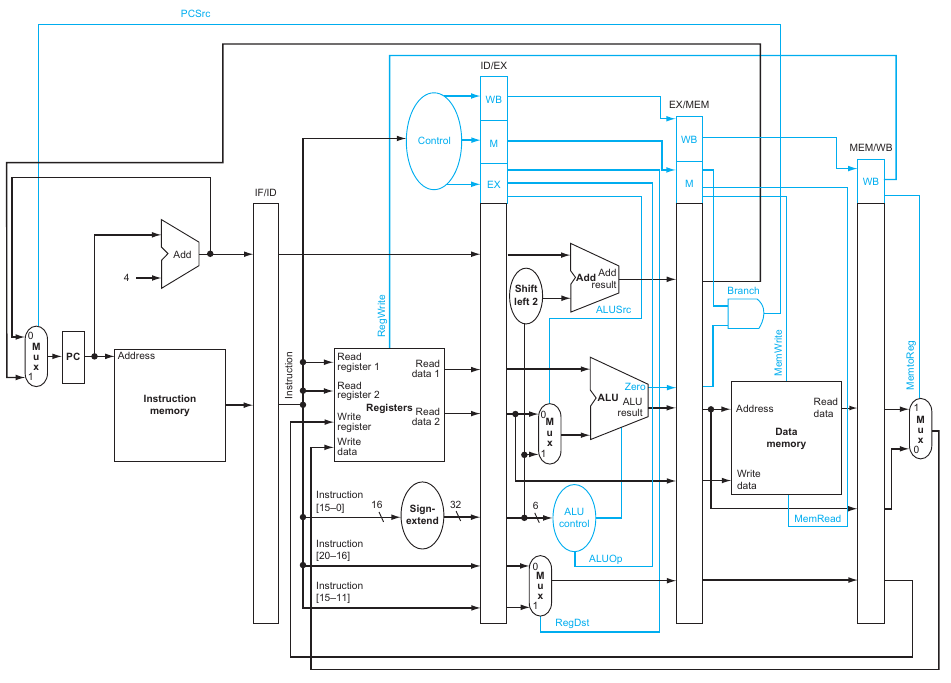
\includegraphics[width=\textwidth]{figure/figure451-mips-segmentado.png}
    \caption{MIPS segmentado.}
    \label{fig:mips-complete}
\end{figure}

\subsubsection{Instruction Fetch (IF)}
Enviar el PC a memoria y buscar la instrucción a ejecutar. Actualizar el PC sumando 4 (cada instrucción es de 4 bytes).

En este módulo, la memoria de programa trabaja con el flanco ascendente del clock.
Por otra parte, el contador de programa y los registros de salida del top utilizan el otro flanco
de clock(descendente).
A su vez, es importante mencionar que para la memoria de programa sintetizada
como Block RAM por la herramienta Vivado, se utilizó el template Xilinx Single Port
Byte-Write Read First RAM.

\newpage
\paragraph{Instruction Memory} 
\hfill \par
Memoria dónde son cargadas las instrucciones del programa.  En cada ciclo, con el PC busca la instrucción que va a ejecutar. Antes de que comienza la ejecución del MIPS existe una etapa de carga, donde desde fuera del MIPS se envían instrucciones a ser escritas a posiciones de memoria.


\subsubsection{Instruction Decode (ID)}
Decodificar la instrucción y acceder a los registros implicados. Analizar valores de los registros por posibles saltos (branches). Extender el signo del valor de offset si es necesario. Calcular posible dirección de salto considerando el offset que se debería incrementar al PC.

Módulo combinacional que decodifica la instrucción que proviene de la etapa Instruction Fetch. De este módulo salen las direcciones de registros rs, rt, rd, reg A y reg B. A su vez, el valor inmediato de la instrucción como también detectar los saltos incondicionales y su respectiva dirección.

\paragraph{Control}
\hfill \par
Es un módulo que genera las señales de control para las etapas EX, MEM y WB para la instrucción correspondiente.

\paragraph{Registers}
\hfill \par
Es el banco de 32 registros de 32 bits cada uno. En el flanco ascendente del clock, se escriben con los valores y las señales de control que provienen de la etapa Write Back. Por otra parte, en el flanco descendente se colocan en la salida los valores que contienen los registros apuntados por las direcciones reg A y reg B.

\newpage
\paragraph{Unidad de detección de riesgos (Hazard Detection Unit)}
\hfill \par
Consiste en la detección de riesgos y parada del procesador en un ciclo. Esto involucra incorporar una unidad de detección de riesgos que actúa en ID impidiendo la carga y lectura de una nueva instrucción.

\subsubsection{Execute (EX)}
La ALU usa los operandos, realizando una de 3 funciones según el tipo de instrucción.
\begin{itemize}
    \item \textbf{Memory reference}: suma el registro base y el offset para formar la
dirección efectiva.

    \item \textbf{Register-Register}: opera según el opcode entre dos registros.

    \item \textbf{Register-Immediate}: opera según el opcode entre un registro y un valor inmediato.
\end{itemize}

\paragraph{ALU Control}
\hfill \par
Genera los bits de control para diferentes tipos de operaciones de la ALU. 

\paragraph{ALU}
\hfill \par
Es un módulo combinacional que efectúa la operación solicitada entre los dos operandos de sus entradas en función de la señal de control ALU Control.

\subsubsection{Memory Access (MEM)} 
Con la dirección efectiva, se realiza el acceso a memoria, tanto sea un “load” o un “store”.

\paragraph{Data Memory}
\hfill \par 
Memoria donde son almacenados los datos del programa.


\subsubsection{Write Back (WB)}
Para instrucciones R o Load, se escribe el resultado en el registro correspondiente.

\subsubsection{Unidad de Cortocircuito (Forwarding Unit)}
Toma operandos fuentes (\textbf{rs} y \textbf{rt}) de la instrucción que se está por ejecutar y los destino (\textbf{rd}) de las instrucciones anteriores y los compara. Si son iguales, adelanta el resultado para no esperar WB. Se hace cortocircuito si las anteriores quieren escribir el registro que estoy por usar.


\begin{figure} [H]
    \centering
    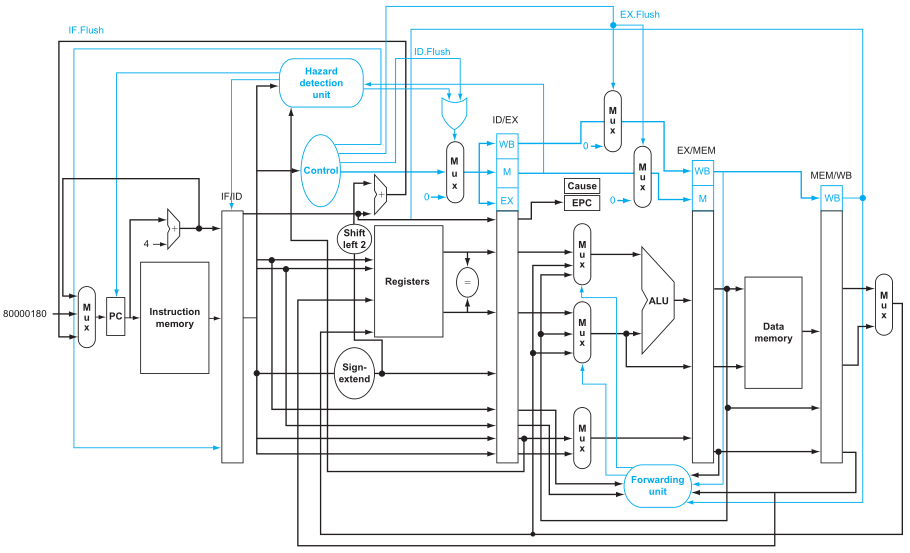
\includegraphics[width=\textwidth]{figure/figure466-mips-finalv2.png}
    \caption{MIPS completo con control de riesgos.}
    \label{fig:mips-complete-control-de-riesgos}
\end{figure}

\section{Ensamblador}
Se desarrolló en Python un script que permite la generación de código binario a partir del Set de instrucciones MIPS. El programa a ejecutar es escrito en un archivo de texto que es utilizado para inicializar la memoria de instrucciones. \\
\textbf{Código assembler}:


\begin{figure}[H]
    \centering
    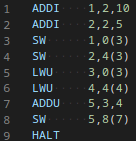
\includegraphics[scale=1.0]{figure/Codigo-Asm.png}
    \caption{Código Assembler a convertir.}
    \label{fig:my_label}
\end{figure}

\noindent \textbf{Salida del ensamblador}:
\begin{figure}[H]
    \centering
    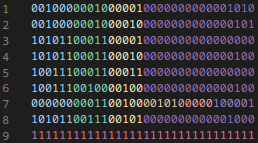
\includegraphics[scale=1.0]{figure/Output-bin.png}
    \caption{Código binario generado a partir del script.}
    \label{fig:my_label}
\end{figure}

\section{Módulo Clock Wizard}
La implementación del proyecto dio como resultado una frecuencia de clock máximo de 32 MHz. A esta frecuencia se cumplieron todas las restricciones de tiempo especificadas como se puede observar en la figura \ref{fig:timing-rep}. Este módulo provee la frecuencia elegida a todos los demás bloques del proyecto.

\begin{figure} [H]
    \centering
    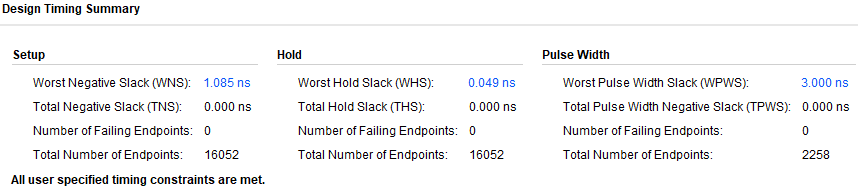
\includegraphics[width=\textwidth]{figure/32MHz-timing-report.png}
    \caption{Resumen de reporte de tiempo a 32MHz.}
    \label{fig:timing-rep}
\end{figure}

\section{Clock Enable}
Se modificó el comportamiento del clock en el procesador MIPS. Este es habilitado mediante una señal de enable para poder realizar una ejecución paso a paso. Dicha señal de enable dura exactamente 1 ciclo de reloj del MIPS cada vez que es pulsado el botón correspondiente para la ejecución.

\section{Test Bench}
Para el diseño del procesador se confeccionó una hoja de donde se encuentra el estado de todas las señales de control frente a cada instrucción.
El testing se realizó primeramente mediante test benches, que permitieron comprobar que la simulación realizara lo esperado. Este proceso se expandió etapa a etapa, hasta completar la simulación del procesador en su totalidad.


Se comprobó que cada una de las instrucciones funcionaran correctamente en diferentes casos planteados.

\begin{figure} [H]
    \centering
    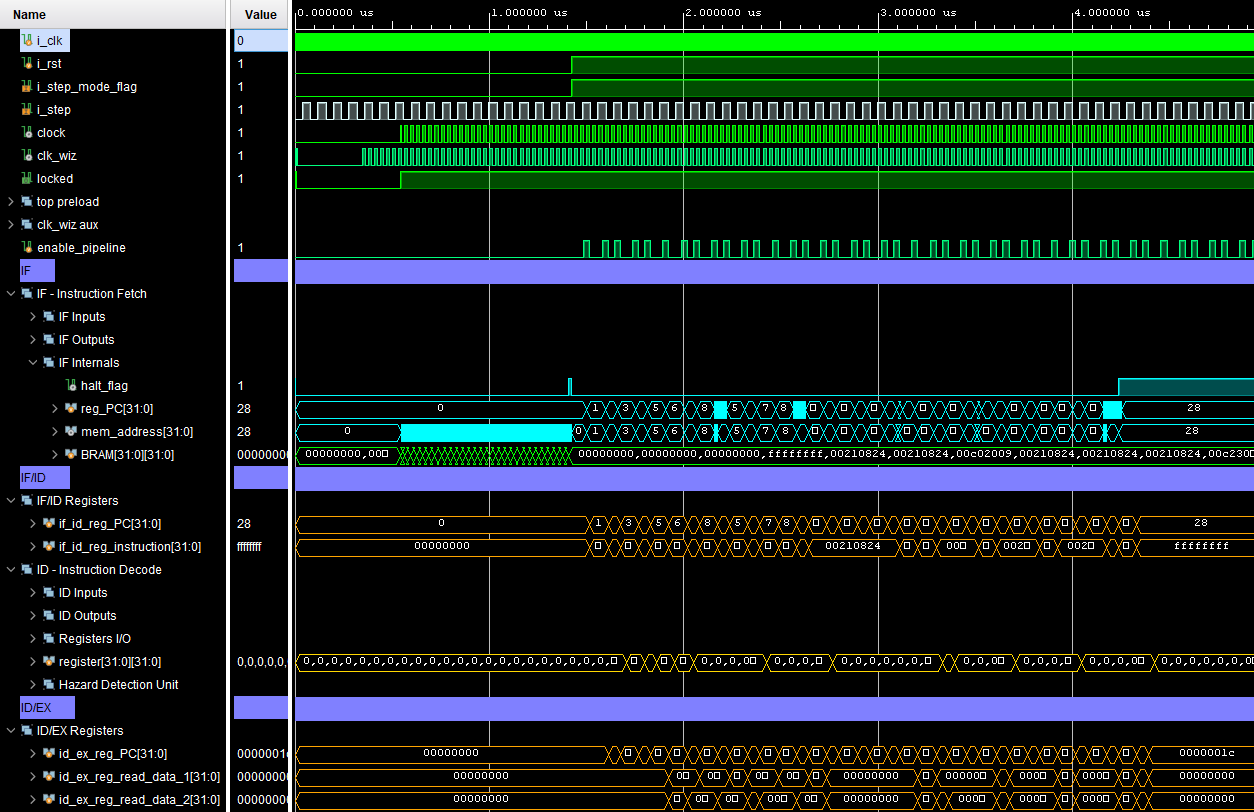
\includegraphics[width=\textwidth]{figure/testbench-wave.png}
    \caption{Wavefile de la ejecución del test 8.}
    \label{fig:test-bench}
\end{figure}

\newpage
\section{Conclusión}
Una vez terminado el práctico, a través de la herramienta Vivado se
obtuvieron las especificaciones en la utilización de los recursos de la FPGA y en la potencia que consume dicho circuito instanciado.

Se logró implementar y probar todas las instrucciones, verificando que no haya conflictos entre todas las posibles acciones que se pueden tomar. 

A demás, la ejecución del MIPS a una frecuencia máxima de 32 MHz. Para aumentar la velocidad de funcionamiento, se debería rediseñar la arquitectura del mismo, debido a los problemas de lógica en cada etapa; un ejemplo puntual de esto, se manifiesta en las escrituras a registros entre flancos consecutivos cuando existe demasiada lógica combinacional entre eventos.

\end{document}

